\documentclass[12pt, openany, oneside]{book}

\usepackage{listings}
\usepackage[dvipsnames]{xcolor}
\usepackage{ctex}
\usepackage{fontspec}
\usepackage{setspace}
\usepackage{tikz}
\usepackage{anyfontsize}
\usepackage{sectsty}
\usepackage{titlesec}
\usepackage{float}
\usepackage[hidelinks]{hyperref}
\usepackage[a4paper]{geometry}
\usepackage{url}
\usepackage{amssymb}
\usepackage{fontawesome5}
\usepackage[most]{tcolorbox}
\usepackage{stackengine}
\usepackage{multirow}
\usepackage[T1]{fontenc}
\usepackage{diagbox}
\usepackage{longtable}
\usepackage{newtxtt}
\usepackage{pgf-umlcd}
\usepackage{bbding}
\usepackage[edges]{forest}
% \usepackage{minted}

\makeatletter
\newcommand{\verbatimfont}[1]{\renewcommand{\verbatim@font}{\ttfamily#1}}
\makeatother

\usetikzlibrary{calc,trees,positioning,arrows,fit,shapes}
\usetikzlibrary{shapes.multipart,chains}
\usetikzlibrary{shadows}

\tikzstyle{startend} = [rectangle, rounded corners, minimum width=3cm, minimum height=1cm, text centered, draw=black, fill=red!30]
\tikzstyle{io}        = [trapezium, trapezium left angle=70, trapezium right angle=110, minimum width=3cm, inner xsep = -15pt, minimum height=1cm, text centered, draw=black, fill=blue!30]
\tikzstyle{process}   = [rectangle, minimum width=3cm, minimum height=1cm, inner ysep=0, text centered, draw=black, fill=orange!30]
\tikzstyle{decision}  = [diamond,shape aspect=2.5, minimum width=3cm, minimum height=1cm, inner xsep=0,text centered, draw=black, fill=green!30]
\tikzstyle{arrow}     = [thick,->,>=stealth]

\def\rlwd{.5pt} \def\rlht{2.2ex} \def\rldp{.5ex}
\def\mydiv#1{~%
  \rule[-\rldp]{\rlwd}{\rlht}%
  \setbox0=\hbox{~#1}%
  \stackunder[\dimexpr\rldp-\rlwd]{~#1}{\rule{\wd0}{\rlwd}}%
}

\definecolor{mycolor}{RGB}{0,128,128}
\newtcbox{\mybox} {
    on line,
    colback=mycolor,
    fontupper=\bfseries\color{white},
    boxrule=0pt,
    arc=5pt, 
    boxsep=0pt, 
    left=2pt, 
    right=2pt, 
    top=5pt, 
    bottom=5pt
}

\setstretch{1.5}
\setlength{\parindent}{0cm}

\geometry{a4paper,top=2.5cm,bottom=2.5cm}

\titleformat{\chapter}{\Huge\Huge\bfseries}{\chaptertitlename\ \thechapter{\ }}{0pt}{\Huge}{}
\titlespacing{\chapter}{0pt}{0pt}{12pt}

\definecolor{dkgreen}{rgb}{0,0.4,0}
\definecolor{gray}{rgb}{0.5,0.5,0.5}
\definecolor{mauve}{rgb}{0.58,0,0.82}
\definecolor{LightGray}{gray}{0.9}

\lstset{
    basicstyle=\linespread{1.3} \fontspec{Consolas},    %  the size of the fonts that are used for the code
	basewidth=0.5em,
    numbers=left,            % where to put the line-numbers
    numberstyle=\color{black},  % the style that is used for the line-numbers
    numbersep=10pt,                  % how far the line-numbers are from the code
    backgroundcolor=\color{white},
    showspaces=false,
    showstringspaces=false,
    showtabs=false,
    frame=single,                   % adds a frame around the code
    rulecolor=\color{black},        % if not set, the frame-color may be changed on line-breaks within not-black text (e.g. commens (green here))
    tabsize=4,                      % sets default tabsize to 2 spaces
    captionpos=t,                   % sets the caption-position to bottom
    breaklines=false,                % sets automatic line breaking
    breakatwhitespace=true,        % sets if automatic breaks should only happen at whitespace
    title=\lstname,                   % show the filename of files included with \lstinputlisting;
    % also try caption instead of title
    numberstyle=\color{black},		% line number color
    keywordstyle=\color{blue},          % keyword style
    commentstyle=\color{dkgreen},       % comment style
    stringstyle=\color{mauve},         % string literal style
    escapeinside={\%*}{*)},            % if you want to add LaTeX within your code
    morekeywords={*,...}               % if you want to add more keywords to the set
}

\begin{document}

\thispagestyle{empty}

\begin{tikzpicture}[overlay,remember picture]
    % Background color
    \fill[
        black!2]
    (current page.south west) rectangle (current page.north east);

    % Rectangles
    \shade[
        left color=Dandelion,
        right color=Dandelion!40,
        transform canvas ={rotate around ={45:($(current page.north west)+(0,-6)$)}}]
    ($(current page.north west)+(0,-6)$) rectangle ++(9,1.5);

    \shade[
        left color=lightgray,
        right color=lightgray!50,
        rounded corners=0.75cm,
        transform canvas ={rotate around ={45:($(current page.north west)+(.5,-10)$)}}]
    ($(current page.north west)+(0.5,-10)$) rectangle ++(15,1.5);

    \shade[
        left color=lightgray,
        rounded corners=0.3cm,
        transform canvas ={rotate around ={45:($(current page.north west)+(.5,-10)$)}}] ($(current page.north west)+(1.5,-9.55)$) rectangle ++(7,.6);

    \shade[
        left color=orange!80,
        right color=orange!60,
        rounded corners=0.4cm,
        transform canvas ={rotate around ={45:($(current page.north)+(-1.5,-3)$)}}]
    ($(current page.north)+(-1.5,-3)$) rectangle ++(9,0.8);

    \shade[
        left color=red!80,
        right color=red!80,
        rounded corners=0.9cm,
        transform canvas ={rotate around ={45:($(current page.north)+(-3,-8)$)}}] ($(current page.north)+(-3,-8)$) rectangle ++(15,1.8);

    \shade[
        left color=orange,
        right color=Dandelion,
        rounded corners=0.9cm,
        transform canvas ={rotate around ={45:($(current page.north west)+(4,-15.5)$)}}]
    ($(current page.north west)+(4,-15.5)$) rectangle ++(30,1.8);

    \shade[
        left color=RoyalBlue,
        right color=Emerald,
        rounded corners=0.75cm,
        transform canvas ={rotate around ={45:($(current page.north west)+(13,-10)$)}}]
    ($(current page.north west)+(13,-10)$) rectangle ++(15,1.5);

    \shade[
        left color=lightgray,
        rounded corners=0.3cm,
        transform canvas ={rotate around ={45:($(current page.north west)+(18,-8)$)}}]
    ($(current page.north west)+(18,-8)$) rectangle ++(15,0.6);

    \shade[
        left color=lightgray,
        rounded corners=0.4cm,
        transform canvas ={rotate around ={45:($(current page.north west)+(19,-5.65)$)}}]
    ($(current page.north west)+(19,-5.65)$) rectangle ++(15,0.8);

    \shade[
        left color=OrangeRed,
        right color=red!80,
        rounded corners=0.6cm,
        transform canvas ={rotate around ={45:($(current page.north west)+(20,-9)$)}}]
    ($(current page.north west)+(20,-9)$) rectangle ++(14,1.2);

    % Year
    % \draw[ultra thick,gray]
    % ($(current page.center)+(5,2)$) -- ++(0,-3cm)
    node[
            midway,
            left=0.25cm,
            text width=5cm,
            align=right,
            black!75
        ]
        {
            % {\fontsize{25}{30} \selectfont \bf ANNUAL \\[10pt] REPORT}
        }
    node[
            midway,
            right=0.25cm,
            text width=6cm,
            align=left,
            orange]
        {
            % {\fontsize{72}{86.4} \selectfont 2020}
        };

    % Title
    \node[align=center] at ($(current page.center)+(0,-5)$)
    {
    {\fontsize{72}{72} \selectfont {{Python}}} \\[2cm]
    {\fontsize{20}{19.2} \selectfont \textcolor{orange}{ \bf 极夜酱}} \\[4pt]
    };
\end{tikzpicture}

\newpage

\pagestyle{plain}
\setcounter{page}{1}
\setcounter{tocdepth}{1}
\tableofcontents

\newpage

\setcounter{page}{1}

\chapter{Hello World!}

\section{Hello World!}

\subsection{编程语言(Programming Language)}

程序是为了让计算机去解决某些问题,它由一系列指令构成。但是计算机并不能理解人类的语言,即使是最简单的,例如“计算一下1+2是多少”。\\

计算机采用的是二进制(binary),也就是只能够理解0和1,因此编程语言用于作为人类与计算机之间沟通的桥梁。

\begin{figure}[H]
	\centering
	
\includegraphics[scale=0.9]{img/Chapter1/1-1/1.png}
\end{figure}

通过使用编程语言来描述解决问题的步骤,从而让计算机一步一步去执行。流程图(flow chat)成为了一种程序的图形化表示方式。\\

\begin{figure}[H]
	\centering
	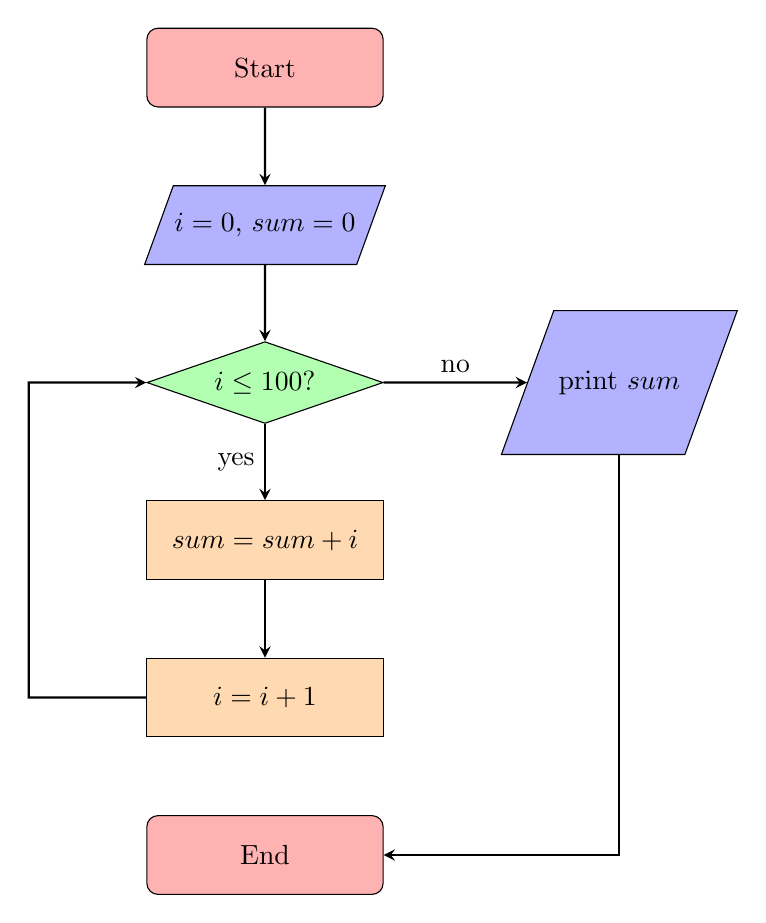
\begin{tikzpicture}[node distance=2cm]
		\node (start) [startend] {Start};
		\node (init) [io, below of=start] {$ i = 0 $, $ sum = 0 $};
		\node (decision)  [decision, below of=init] {$ i \le 100 $?};
		\node (accumulation) [process, below of=decision] {$ sum = sum + i $};
		\node (update) [process, below of=accumulation] {$ i = i + 1 $};
		\node (output) [io, right of=decision, xshift=2.5cm] {print $ sum $};
		\node (end) [startend, below of=update] {End};

		\draw [arrow] (start) -- (init);
		\draw [arrow] (init) -- (decision);
		\draw [arrow] (decision) -- node[anchor=east] {yes } (accumulation);
		\draw [arrow] (accumulation) -- (update);
		\draw [arrow] (update) -- (-3,-8) -- (-3,-4) -- (decision);
		\draw [arrow] (decision) -- node[anchor=south] {no} (output);
		\draw [arrow] (output) |- (end);
	\end{tikzpicture}
	\caption{计算$ \sum_{i=1}^{100} i $的流程图}
\end{figure}

\vspace{0.5cm}

\subsection{Hello World!}

Hello World是学习编程的第一个程序,它的作用是向屏幕输出"Hello World!"。\\

\mybox{Hello World!}

\begin{lstlisting}[language=Python]
print("Hello World!")
\end{lstlisting}

\begin{tcolorbox}
	\mybox{运行结果}
	\begin{verbatim}
Hello World!
	\end{verbatim}
\end{tcolorbox}

不同编程语言的Hello World写法大同小异,可以看出编程语言的基本结构是相似的。\\

\mybox{C}

\begin{lstlisting}[language=C]
#include <stdio.h>

int main() {
	printf("Hello World!\n");
	return 0;
}
\end{lstlisting}

\vspace{0.5cm}

\mybox{C++}

\begin{lstlisting}[language=C++]
#include <iostream>

using namespace std;

int main() {
	cout << "Hello World!" << endl;
	return 0;
}
\end{lstlisting}

\vspace{0.5cm}

\mybox{Java}

\begin{lstlisting}[language=Java]
public class HelloWorld {
    public static void main(String[] args) {
        System.out.println("Hello World!");
    }
}
\end{lstlisting}

\vspace{0.5cm}

\subsection{注释(Comment)}

注释就是对代码的解释和说明,它并不会程序所执行。注释能提高程序的可读性,让人更加容易了解代码的功能。\\

注释一般分为单行注释和多行注释:

\begin{enumerate}
	\item 单行注释:以\#开头,该行之后的内容视为注释。
	\item 多行注释:以"""开头,"""结束,中间的内容视为注释。
\end{enumerate}

\vspace{0.5cm}

\mybox{注释}

\begin{lstlisting}[language=Python]
"""
    Author: Terry
    Date: 2022/11/16
"""
print("Hello World!")       # display "Hello World!"
\end{lstlisting}

\newpage

\section{数据类型}

\subsection{数据类型(Data Types)}

在计算机中,每个数据一般都有一个对应的类型,基础数据类型包括:

\begin{enumerate}
	\item 数值型
	      \begin{itemize}
		      \item 整数int
		      \item 浮点数float
		      \item 复数complex
	      \end{itemize}

	\item 文本型
	      \begin{itemize}
		      \item 字符串str
	      \end{itemize}

	\item 布尔型bool

	\item 数据结构
	      \begin{itemize}
		      \item 列表list
		      \item 元组tuple
		      \item 集合set
		      \item 字典dict
	      \end{itemize}
\end{enumerate}

\vspace{0.5cm}

\subsection{变量(Variable)}

变量是用来存储数据的内存空间,每个变量都有一个类型,使用type()函数可以查看变量的类型。

\vspace{-0.5cm}

\begin{lstlisting}[language=Python]
num = 10;
print(type(num))	# <class 'int'>
salary = 8232.56;
print(type(salary))	# <class 'float'>
\end{lstlisting}

\vspace{0.5cm}

变量的命名需要符合规范:

\begin{enumerate}
	\item 由字母、数字和下划线组成,不能以数字开头
	\item 不可以使用编程语言中预留的关键字
	\item 使用英语单词,顾名思义
\end{enumerate}

关键字是编程语言内置的一些名称,具有特殊的用处和意义,因此不应该作为变量名,防止产生歧义。\\

\begin{table}[H]
	\centering
	\setlength{\tabcolsep}{5mm}{
		\begin{tabular}{|c|c|c|c|c|}
			\hline
			False  & None  & True   & and      & as      \\
			\hline
			assert & break & class  & continue & def     \\
			\hline
			del    & elif  & else   & except   & finally \\
			\hline
			for    & from  & global & if       & import  \\
			\hline
			in     & is    & lambda & nonlocal & not     \\
			\hline
			or     & pass  & raise  & return   & try     \\
			\hline
			while  & with  & yield  &          &         \\
			\hline
		\end{tabular}
	}
	\caption{关键字}
\end{table}

\newpage

\section{输入输出函数}

\subsection{print()}

print()的功能是向屏幕输出指定格式的文本,但是有些需要输出的字符在编程语言中具有特殊含义,因此这些特殊的字符,需要经过转义后输出。\\

\begin{table}[H]
	\centering
	\setlength{\tabcolsep}{5mm}{
		\begin{tabular}{|c|c|}
			\hline
			\textbf{转义字符}      & \textbf{描述}                \\
			\hline
			\lstinline|\\| & 反斜杠\lstinline|\| \\
			\hline
			\lstinline|\'| & 单引号\lstinline|'| \\
			\hline
			\lstinline|\"| & 双引号\lstinline|"| \\
			\hline
			\lstinline|\n| & 换行                         \\
			\hline
			\lstinline|\t| & 制表符                       \\
			\hline
		\end{tabular}
	}
	\caption{转义字符}
\end{table}

\mybox{转义字符}

\begin{lstlisting}[language=Python]
print("\"Hello\nWorld\"")
\end{lstlisting}

\begin{tcolorbox}
	\mybox{运行结果}
	\begin{verbatim}
"Hello
World"
	\end{verbatim}
\end{tcolorbox}

除了直接使用print()输出一个变量的值外,还可以在print()中使用对应类型的占位符。\\

\begin{table}[H]
	\centering
	\setlength{\tabcolsep}{5mm}{
		\begin{tabular}{|c|c|}
			\hline
			\textbf{数据类型} & \textbf{占位符} \\
			\hline
			int               & \%d             \\
			\hline
			float             & \%f             \\
			\hline
			str               & \%s             \\
			\hline
		\end{tabular}
	}
	\caption{占位符}
\end{table}

\vspace{0.5cm}

\mybox{长方形面积}

\begin{lstlisting}[language=Python]
length = 10
width = 5
area = length * width
print("Area = %d * %d = %.2f" % (length, width, area))
\end{lstlisting}

\begin{tcolorbox}
	\mybox{运行结果}
	\begin{verbatim}
Area = 10 * 5 = 50.00
	\end{verbatim}
\end{tcolorbox}

另一种输出的方式是使用f-string,它可以在字符串中直接使用变量的值。

\vspace{-0.5cm}

\begin{lstlisting}[language=Python]
print(f"Area = {length} * {width} = {area:.2f}")
\end{lstlisting}

在默认情况下,print()函数输出数据后,会以换行作为结束符。如果不希望使用换行作为结束符,则可以在print()函数中追加一个end参数。\\

\mybox{等比数列}

\begin{lstlisting}[language=Python]
num1 = 1
num2 = 2
num3 = 4
num4 = 8
print(num1, end=', ')
print(num2, end=', ')
print(num3, end=', ')
print(num4, end='...')
\end{lstlisting}

\begin{tcolorbox}
	\mybox{运行结果}
	\begin{verbatim}
1, 2, 4, 8...
\end{verbatim}
\end{tcolorbox}

\vspace{0.5cm}

\subsection{input()}

有时候一些数据需要从键盘输入,input()可以读取用户输入,并赋值给相应的变量。\\

input()读取到的数据类型是str,通过转换函数可以将其转换为其它类型。\\

\mybox{圆面积}

\begin{lstlisting}[language=Python]
import math

r = float(input("Radius: "))
area = math.pi * r ** 2
print("Area = %.2f" % area)
\end{lstlisting}

\begin{tcolorbox}
	\mybox{运行结果}
	\begin{verbatim}
Radius: 5
Area = 78.54
	\end{verbatim}
\end{tcolorbox}

math模块中定义了一些常用的数学函数,例如pow(x, y)可用于计算$ x $的$ y $次方。\\

\newpage

\section{表达式}

\subsection{算术运算符}

整除运算符//用于计算两个数相除的整数部分,例如21 // 4 = 5。\\

取模(modulo)运算符\%用于计算两个整数相除之后的余数,例如22 \% 3 = 1、4 \% 7 = 4。\\

\mybox{逆序三位数}

\begin{lstlisting}[language=Python]
num = int(input("Enter a 3-digit integer: "))
a = num // 100
b = num // 10 % 10
c = num % 10
print("Reversed:", c * 100 + b * 10 + a)
\end{lstlisting}

\begin{tcolorbox}
	\mybox{运行结果}
	\begin{verbatim}
Enter a 3-digit integer: 520
Reversed: 25
	\end{verbatim}
\end{tcolorbox}

\vspace{0.5cm}

\subsection{复合运算符}

使用复合运算符可以使表达式更加简洁。例如\lstinline|a = a + b|可以写成\lstinline|a += b|,-=、*=、/=、\%=等复合运算符的使用方式同理。\\

\mybox{字符串拼接}

\begin{lstlisting}[language=Python]
s = "Hello" + "World"
s += "!"
print(s)
\end{lstlisting}

\begin{tcolorbox}
	\mybox{运行结果}
	\begin{verbatim}
HelloWorld!
\end{verbatim}
\end{tcolorbox}

\newpage
\chapter{判断}

\section{逻辑运算符}

\subsection{逻辑运算符}

Python中逻辑运算符有三种:

\begin{enumerate}
	\item 逻辑与and:当多个条件同时为真,结果为真。
	      \begin{table}[H]
		      \centering
		      \setlength{\tabcolsep}{5mm}{
			      \begin{tabular}{|c|c|c|}
				      \hline
				      \textbf{条件1} & \textbf{条件2} & \textbf{条件1 and 条件2} \\
				      \hline
				      T              & T              & T                        \\
				      \hline
				      T              & F              & F                        \\
				      \hline
				      F              & T              & F                        \\
				      \hline
				      F              & F              & F                        \\
				      \hline
			      \end{tabular}
		      }
		      \caption{逻辑与}
	      \end{table}

	\item 逻辑或or:多个条件有一个为真时,结果为真。
	      \begin{table}[H]
		      \centering
		      \setlength{\tabcolsep}{5mm}{
			      \begin{tabular}{|c|c|c|}
				      \hline
				      \textbf{条件1} & \textbf{条件2} & \textbf{条件1 or 条件2} \\
				      \hline
				      T              & T              & T                       \\
				      \hline
				      T              & F              & T                       \\
				      \hline
				      F              & T              & T                       \\
				      \hline
				      F              & F              & F                       \\
				      \hline
			      \end{tabular}
		      }
		      \caption{逻辑或}
	      \end{table}

	\item 逻辑非not:条件为真时,结果为假;条件为假时,结果为真。
	      \begin{table}[H]
		      \centering
		      \setlength{\tabcolsep}{5mm}{
			      \begin{tabular}{|c|c|}
				      \hline
				      \textbf{条件} & \textbf{not 条件} \\
				      \hline
				      T             & F                 \\
				      \hline
				      F             & T                 \\
				      \hline
			      \end{tabular}
		      }
		      \caption{逻辑非}
	      \end{table}
\end{enumerate}

\newpage

\section{if}

\subsection{if}

分支结构最大特征就是可以进行指定条件的判断处理,关键字为if、elif、else。\\

每一个满足条件之后的语句都可以有多条,并且在Python里面是利用缩进来确定语句的关系。使用逻辑运算符可以进行若干个条件的连接。

\subsubsection{单分支}

\vspace{-1cm}

\begin{lstlisting}[language=Python]
age = 15
if 0 < age < 18:
    print("未成年")
\end{lstlisting}

\subsubsection{双分支}

\vspace{-1cm}

\begin{lstlisting}[language=Python]
age = 30
if 0 < age < 18:
    print("未成年人")
else:
    print("成年人")
\end{lstlisting}

\subsubsection{多分支}

\vspace{-1cm}

\begin{lstlisting}[language=Python]
score = 76

if 90 <= score <= 100:
    print("优秀")
elif score >= 60:
    print("合格")
else:
    print("不合格")
\end{lstlisting}

\vspace{0.5cm}

\mybox{判断整数奇偶}

\begin{lstlisting}[language=Python]
num = int(input("输入一个正整数:"))

if num > 0:
    if num % 2 == 0:
        print("%d是偶数" % num)
    else:
        print("%d是奇数" % num)
\end{lstlisting}

\begin{tcolorbox}
	\mybox{运行结果}
	\begin{verbatim}
输入一个正整数:66
66是偶数
\end{verbatim}
\end{tcolorbox}

\newpage

\section{断言}

\subsection{断言(Assertion)}

设置断言表达式后,当满足条件时程序正常执行,当断言失败时,程序会中断执行。在进行断言时可以配置错误的提示信息,否则很难知道那块代码出现了错误。\\

通过断言可以直接查找出程序的错误,但从另外一个角度来讲,断言由于不受到程序逻辑的控制,可能会造成许多的额外的问题,在实际的开发之中慎用。\\

\mybox{断言}

\begin{lstlisting}[language=Python]
import math

print("计算三角形面积")
a = float(input("第一条边:"))
b = float(input("第二条边:"))
c = float(input("第三条边:"))

assert a + b > c, "边长不合法"
assert a + c > b, "边长不合法"
assert b + c > a, "边长不合法"

p = (a + b + c) / 2     # 半周长
area = math.sqrt(p * (p-a) * (p-b) * (p-c)) # 海伦公式
print("面积 = %.2f" % area)
\end{lstlisting}

\begin{tcolorbox}
	\mybox{运行结果}
	\begin{verbatim}
计算三角形面积
第一条边:1
第二条边:1
第三条边:2
AssertionError: 边长不合法
\end{verbatim}
\end{tcolorbox}

\newpage
\chapter{循环}

\section{while}

\subsection{while}

while循环会对条件进行判断,如果条件成立,就会执行循环体,然后再次判断条件,直到条件不成立。\\

while循环的次数由循环变量的变化决定,因此while循环一般都包括对循环变量的初值、判断和更新。

\vspace{-0.5cm}

\begin{lstlisting}[language=Python]
i = 1			# initial value
while i <= 5:	# condition
	print("In loop: i =", i)
	i += 1		# update
print("After loop: i =", i)
\end{lstlisting}

while循环的特点是先判断、再执行,因此循环体有可能会执行一次或多次,也有可能一次也不会执行。\\

\mybox{平均身高}

\begin{lstlisting}[language=Python]
NUM_PEOPLE = 5

total = 0

i = 1
while i <= NUM_PEOPLE:
	height = float(input("Enter person %d's height: " % i))
	total += height
	i += 1

average = total / NUM_PEOPLE
print("Average height: %.2f" % average)
\end{lstlisting}

\begin{tcolorbox}
	\mybox{运行结果}
	\begin{verbatim}
Enter person 1's height: 160.8
Enter person 2's height: 175.2
Enter person 3's height: 171.2
Enter person 4's height: 181.3
Enter person 5's height: 164
Average height: 170.50
\end{verbatim}
\end{tcolorbox}

\vspace{0.5cm}

\mybox{整数位数}

\begin{lstlisting}[language=Python]
num = int(input("Enter an integer: "))
n = 0

while num != 0:
	num //= 10
	n += 1

print("Digits:", n)
\end{lstlisting}

\begin{tcolorbox}
	\mybox{运行结果}
	\begin{verbatim}
Enter an integer: 123
Digits: 3
\end{verbatim}
\end{tcolorbox}

\vspace{0.5cm}

\mybox{猜数字}

\begin{lstlisting}[language=Python]
import random

answer = random.randint(1, 100)
cnt = 0

while True:
	num = int(input("Guess a number: "))
	cnt += 1

	if num > answer:
		print("Too high")
	elif num < answer:
		print("Too low")
	else:
		break

print("Correct! You guessed %d times." % cnt)
\end{lstlisting}

\begin{tcolorbox}
	\mybox{运行结果}
	\begin{verbatim}
Guess a number: 50
Too high
Guess a number: 25
Too low
Guess a number: 37
Too low
Guess a number: 43
Too high
Guess a number: 40
Too high
Guess a number: 38
Too low
Guess a number: 39
Correct! You guessed 7 times.
\end{verbatim}
\end{tcolorbox}

\newpage

\section{for}

\subsection{for}

while循环将循环变量的初值、条件和更新写在了三个地方,但是这样不容易明显地看出循环变量的变化。\\

for循环在一行内就可以清晰地表示出循环的次数,因此对于指定次数的循环一般更多地会采用for循环,而对于不确定次数的一般会采用while循环。\\

range()函数能够生成指定范围的整数序列:

\vspace{-0.5cm}

\begin{lstlisting}[language=Python]
for i in range(5):
    print(i, end=' ')		# 0 1 2 3 4

for i in range(10, 15):
	print(i, end=' ')		# 10 11 12 13 14

for i in range(1, 10, 2):
	print(i, end=' ')		# 1 3 5 7 9
\end{lstlisting}

\vspace{0.5cm}

\mybox{累加}

\begin{lstlisting}[language=Python]
sum = 0
for i in range(1, 101):
	sum += i
print("Sum =", sum)
\end{lstlisting}

\begin{tcolorbox}
	\mybox{运行结果}
	\begin{verbatim}
Sum = 5050
\end{verbatim}
\end{tcolorbox}

\vspace{0.5cm}

\mybox{斐波那契数列}

\begin{figure}[H]
	\centering
	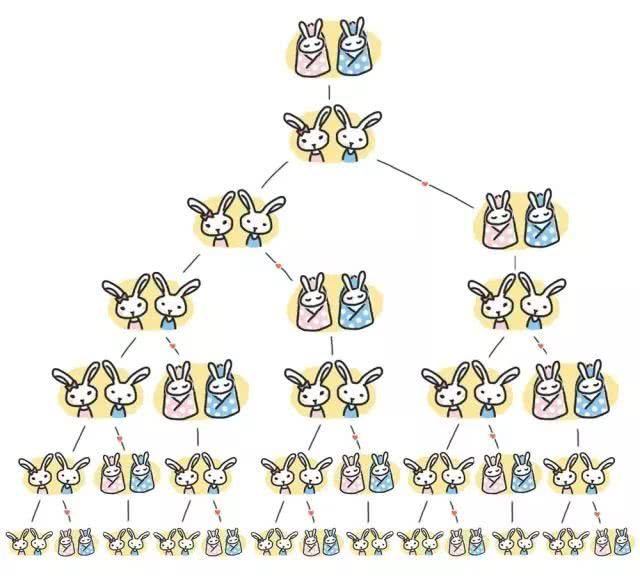
\includegraphics[scale=0.5]{img/Chapter3/3-2/1.png}
\end{figure}

\begin{lstlisting}[language=Python]
n = int(input("Enter the number of terms: "))

if n == 1:
	print(1)
elif n == 2:
	print(1, 1)
else:
	num1 = 1
	num2 = 1
	print(1, 1, end=' ')
	for i in range(3, n + 1):
		val = num1 + num2
		print(val, end=' ')
		num1 = num2
		num2 = val
	print()
\end{lstlisting}

\begin{tcolorbox}
	\mybox{运行结果}
	\begin{verbatim}
Enter the number of terms: 10
1 1 2 3 5 8 13 21 34 55
\end{verbatim}
\end{tcolorbox}

\vspace{0.5cm}

\subsection{嵌套循环}

循环也可以嵌套使用,外层循环每执行一次,内层循环就会执行多次。

\vspace{-0.5cm}

\begin{lstlisting}[language=Python]
for i in range(2):
	for j in range(3):
		print("i = %d, j = %d" % (i, j))
\end{lstlisting}

\begin{tcolorbox}
	\mybox{运行结果}
	\begin{verbatim}
i = 0, j = 0
i = 0, j = 1
i = 0, j = 2
i = 1, j = 0
i = 1, j = 1
i = 1, j = 2
\end{verbatim}
\end{tcolorbox}

\vspace{0.5cm}

\mybox{九九乘法表}\\

\begin{table}[H]
	\centering
	\setlength{\tabcolsep}{1.5mm}{
		\begin{tabular}{|c|c|c|c|c|c|c|c|c|}
			\hline
			1*1=1 & 1*2=2  & 1*3=3  & 1*4=4  & 1*5=5  & 1*6=6  & 1*7=7  & 1*8=8  & 1*9=9  \\
			\hline
			2*1=2 & 2*2=4  & 2*3=6  & 2*4=8  & 2*5=10 & 2*6=12 & 2*7=14 & 2*8=16 & 2*9=18 \\
			\hline
			3*1=3 & 3*2=6  & 3*3=9  & 3*4=12 & 3*5=15 & 3*6=18 & 3*7=21 & 3*8=24 & 3*9=27 \\
			\hline
			4*1=4 & 4*2=8  & 4*3=12 & 4*4=16 & 4*5=20 & 4*6=24 & 4*7=28 & 4*8=32 & 4*9=36 \\
			\hline
			5*1=5 & 5*2=10 & 5*3=15 & 5*4=20 & 5*5=25 & 5*6=30 & 5*7=35 & 5*8=40 & 5*9=45 \\
			\hline
			6*1=6 & 6*2=12 & 6*3=18 & 6*4=24 & 6*5=30 & 6*6=36 & 6*7=42 & 6*8=48 & 6*9=54 \\
			\hline
			7*1=7 & 7*2=14 & 7*3=21 & 7*4=28 & 7*5=35 & 7*6=42 & 7*7=49 & 7*8=56 & 7*9=63 \\
			\hline
			8*1=8 & 8*2=16 & 8*3=24 & 8*4=32 & 8*5=40 & 8*6=48 & 8*7=56 & 8*8=64 & 8*9=72 \\
			\hline
			9*1=9 & 9*2=18 & 9*3=27 & 9*4=36 & 9*5=45 & 9*6=54 & 9*7=63 & 9*8=72 & 9*9=81 \\
			\hline
		\end{tabular}
	}
\end{table}

\begin{lstlisting}[language=Python]
for i in range(1, 10):
    for j in range(1, 10):
        print("%d*%d=%d\t" % (i, j, i * j), end='')
    print()
\end{lstlisting}

\vspace{0.5cm}

\mybox{打印图案}

\begin{lstlisting}
*
**
***
****
*****
\end{lstlisting}

\begin{lstlisting}[language=Python]
for i in range(1, 6):
	for j in range(1, i + 1):
		print("*", end='')
	print()
\end{lstlisting}

\newpage

\section{break or continue?}

\subsection{break}

break可用于跳出当前的switch或循环结构。在一些情况下,在循环的中途已经完成了某个目标,没有必要再进行剩余的循环,这时就可以使用break跳出循环。\\

例如在判断一个数$ n $是否为素数时,利用循环逐个判断$ 2 \sim n - 1 $之间的数是否能整除$ n $。只要发现其中有一个数能整除$ n $,就证明$ n $不是素数,可以跳出循环,不必再进行剩余的检查。\\

\mybox{素数}

\begin{lstlisting}[language=Python]
import math

n = int(input("Enter an integer: "))

is_prime = True
for i in range(2, int(math.sqrt(n)) + 1):
	if n % i == 0:
		is_prime = False
		break

if is_prime:
	print(n, "is a prime number")
else:
	print(n, "is not a prime number")
\end{lstlisting}

\begin{tcolorbox}
	\mybox{运行结果}
	\begin{verbatim}
Enter an integer: 17
17 is a prime number
\end{verbatim}
\end{tcolorbox}

\vspace{0.5cm}

\subsection{continue}

continue与break使用方法类似,但是它并不是跳出循环,而是跳过本轮循环,直接开始下一轮循环。\\

\mybox{正数平方和}

\begin{lstlisting}[language=Python]
n = 10
print("Enter %d integers: " % n)

sum_square = 0
for i in range(n):
	num = int(input())
	if num < 0:
		continue
	sum_square += num * num

print("Sum of squares of positive integers:", sum_square)
\end{lstlisting}

\begin{tcolorbox}
	\mybox{运行结果}
	\begin{verbatim}
Enter 10 integers: 
5 
7
-2
0
4
-4
-9
3
9
5
Sum of squares of positive integers: 205
\end{verbatim}
\end{tcolorbox}

\newpage

\end{document}